\documentclass[11pt]{article}
\usepackage[T1]{fontenc}
\usepackage{lmodern}
\usepackage[a4paper,margin=27mm]{geometry}
\usepackage{amsmath,amssymb,amsthm,mathtools}
\usepackage{microtype,booktabs,array}
\usepackage{xcolor,tikz}
\usetikzlibrary{arrows.meta,positioning,calc,fit,backgrounds}
\usepackage{caption}
\usepackage{placeins}
\usepackage{needspace}
\usepackage{url}
\usepackage[hidelinks]{hyperref}
\hypersetup{pdftitle={An inverse theorem for extremal generalized Narkiewicz sequences over C3 cubed},pdfauthor={John Fairfax-Ball}}
\pdfinfoomitdate=1
\pdftrailerid{}
\pdfsuppressptexinfo=-1
\newtheorem{theorem}{Theorem}[section]
\newtheorem{proposition}[theorem]{Proposition}
\newtheorem{lemma}[theorem]{Lemma}
\newtheorem{corollary}[theorem]{Corollary}
\theoremstyle{definition}
\newtheorem{definition}[theorem]{Definition}
\newtheorem{example}[theorem]{Example}
\theoremstyle{remark}
\newtheorem{remark}[theorem]{Remark}
\newcommand{\F}{\mathbb F}
\newcommand{\supp}{\operatorname{supp}}
\newcommand{\sig}{\sigma}
\newcommand{\sfreetext}{short-zero-sum-free}
\definecolor{inkblue}{HTML}{245B73}
\definecolor{warm}{HTML}{A66518}
\tikzset{token/.style={circle,draw,minimum size=6mm,inner sep=0pt,font=\small},
  flow/.style={-{Latex[length=2mm]},thick},
  box/.style={draw,rounded corners=2pt,align=center,inner sep=6pt}}
\captionsetup{font=small,labelfont=bf}
\setlength{\emergencystretch}{1em}
\title{An inverse theorem for extremal generalized\\ Narkiewicz sequences over $C_3^3$}
\author{John Fairfax-Ball}
\date{}

\begin{document}
\maketitle
\begin{abstract}
Let $G=(\mathbb Z/3\mathbb Z)^3$. A short zero-sum witness in an indexed
sequence over $G\setminus\{0\}$ is a nonempty set of at most three positions
whose entries sum to zero. The generalized Narkiewicz threshold for two
such witnesses having a nonzero intersection sum is known to be $25$.
We prove the complete inverse statement at length $24$: every pair of
short zero-sum witnesses has zero intersection sum if and only if, up to
a permutation of the original positions, the sequence is $U^3$, where
$U$ consists of eight distinct nonzero elements and has no short zero sum.
Thus the known threefold constructions exhaust the extremal sequences.
The necessity proof combines the published packing and representative-deletion
method with short-free residual structure. Swapping representatives forces
constant blocks in the length-$16$ residual case; the uniquely determined
singleton of a length-$15$ residual excludes the remaining packing case.
\end{abstract}

\noindent\textbf{Keywords:} inverse zero-sum problem; generalized Narkiewicz constant;
extremal sequence; positional intersection.\\
\textbf{Mathematics Subject Classification (2020):} 11B75, 11B30.

\section{Introduction}
Zero-sum thresholds specify how many terms force a prescribed additive
configuration. Their inverse problems ask which sequences avoid that
configuration at the last possible length. For intersection conditions on
zero-sum subsequences, an inverse theorem must control both multiplicities
and the positions of the witnesses: retaining only the support discards part
of the hypothesis.

Gao, Hui, Li, Li, Qu and Zhong~\cite{Gao2024} introduced generalized
Narkiewicz constants using pairs of zero-sum subsequences whose intersection
has nonzero sum. The intersection is taken over the original indices.
For the short-zero-sum invariant they proved
\begin{equation}\label{eq:threshold}
  \eta^N(C_3^3)=25
\end{equation}
and supplied extremal examples of the form $U^3$ with $|U|=8$.
The direct threshold and this construction are already published; see
\cite[Lemma 3.3(2)--(3) and Theorem 3.6(4)]{Gao2024}.
Here we prove that every extremal sequence has precisely that form.

Write $G=C_3^3=\F_3^3$. If $S=(a_p)_{p\in P}$ is a sequence indexed by a
finite set $P$, and $I\subseteq P$, put $\sig_S(I)=\sum_{p\in I}a_p$.
Call $I$ a \emph{short zero-sum witness} when
$1\leq |I|\leq3$ and $\sig_S(I)=0$.
The empty intersection has sum zero. A sequence is \emph{short-free}
if it has no short zero-sum witness, and \emph{squarefree} if its entries
are pairwise distinct.

\Needspace{14\baselineskip}
\begin{theorem}\label{thm:main}
Let $P$ be any set of cardinality $24$, and let $S=(a_p)_{p\in P}$ with
$a_p\in G\setminus\{0\}$ for every $p$. The following are equivalent.
\begin{enumerate}
\item For every pair $I,J\subseteq P$ of short zero-sum witnesses,
\begin{equation}\label{eq:avoid}
                    \sig_S(I\cap J)=0.
\end{equation}
\item There are eight distinct nonzero elements $u_1,\ldots,u_8$ such that
$U=u_1\cdots u_8$ is short-free, and a bijection
$\phi:\{1,\ldots,8\}\times\{1,2,3\}\longrightarrow P$ satisfying
\begin{equation}\label{eq:permutation}
                  a_{\phi(i,j)}=u_i\qquad(1\leq i\leq8,\ 1\leq j\leq3).
\end{equation}
\end{enumerate}
Equivalently, $S=U^3$ as a multisequence, or after a permutation of all
$24$ original positions.
\end{theorem}

The quantifier in part~(1) permits $I=J$, when the condition is automatic.
It is therefore the exact negation of having two innerly
non-zero-sum-joint short zero-sum subsequences in the terminology of
\cite{Gao2024}. The theorem does not say that $S$ is short-free: in the
conclusion, each three-position fibre is itself a short zero sum.

The substance of the inverse conclusion is that arbitrary multiplicities
and possible two-term zero sums cannot survive at length $24$.
We retain the packing method from the proof of
\cite[Lemma 3.3(3)]{Gao2024}, and use the rank-three residual results of
Fan, Gao, Wang, Zhong and Zhuang~\cite{Fan2012}. Equality bookkeeping leaves
four packing signatures. Universal choice of deleted representatives then
forces eight constant triples in three of these cases and contradicts the
fourth. The residual profile and completion argument used below are already
present in the proof of \cite[Lemma 27(3)]{Fan2012}; the contribution here
is their use in the complete inverse argument, particularly the interaction
between two independently variable packed blocks.

Section~\ref{sec:examples} gives concrete examples and explains the positional
condition. Section~\ref{sec:packing} obtains the four signatures.
Sections~\ref{sec:eight} and~\ref{sec:nine} settle the two residual lengths,
and Section~\ref{sec:completion} completes both directions of the theorem.
Figures depict finite sets and multiplicities exactly; none is evidence in
place of the accompanying proof.

\section{Preliminaries and worked examples}\label{sec:examples}
We write sequences multiplicatively, even though $G$ is additive. Thus
$a^3$ means three occurrences of $a$, $v_a(S)$ is its multiplicity, and
$\supp(S)=\{a:v_a(S)>0\}$. The notation $Sx^{-1}$ removes one specified
occurrence with value $x$; it is not multiplication by a group inverse.
We write $\sig(S)$ for the sum of all entries. Whenever two subsequences
are compared, their original position sets are retained.

\subsection{Why positions matter}
\begin{example}[One extra copy]\label{ex:four}
Fix any $a\neq0$. The sequence $a^3$ has exactly one short zero-sum
witness, namely all three positions. In $a^4$, the witnesses
$I=\{1,2,3\}$ and $J=\{2,3,4\}$ have intersection sum $2a=-a\neq0$.
Thus every sequence satisfying~\eqref{eq:avoid} has $v_a(S)\leq3$.
Both sequences have the same one-element support, so their different
behaviour is invisible at the support level.
\end{example}

\begin{figure}[htbp]
\centering
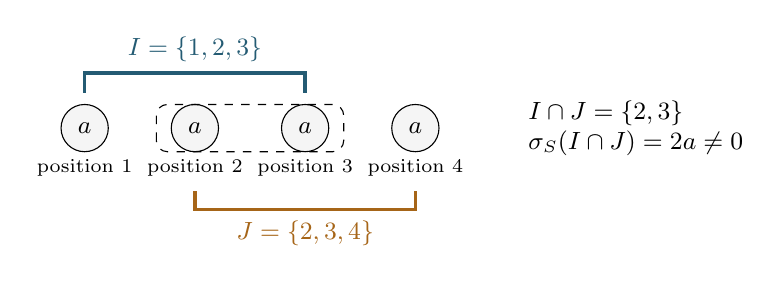
\begin{tikzpicture}[x=1.4cm,y=1cm]
\foreach \i in {1,...,4} {
  \node[token,fill=gray!8] (p\i) at (\i,0) {$a$};
  \node[font=\scriptsize] at (\i,-.5) {position $\i$};}
\draw[inkblue,very thick] (1,.45)--(1,.7)--(3,.7)--(3,.45);
\node[inkblue,font=\small] at (2,1) {$I=\{1,2,3\}$};
\draw[warm,very thick] (2,-.8)--(2,-1.03)--(4,-1.03)--(4,-.8);
\node[warm,font=\small] at (3,-1.34) {$J=\{2,3,4\}$};
\draw[dashed,rounded corners] (1.65,-.3) rectangle (3.35,.3);
\node[align=left,font=\small] at (6,0) {$I\cap J=\{2,3\}$\\$\sig_S(I\cap J)=2a\neq0$};
\end{tikzpicture}
\caption{A forbidden positional overlap in $a^4$. The two witnesses have
the same value-multisequence $a^3$ but different sets of positions.}
\label{fig:overlap}
\end{figure}

\begin{example}[A two-term witness can be allowed]\label{ex:pair}
The two-position sequence $a(-a)$ satisfies~\eqref{eq:avoid}: its only
short zero-sum witness is the entire pair. By contrast, for
$(a,-a,a)$ the witnesses $\{1,2\}$ and $\{2,3\}$ intersect in a
single position of value $-a\neq0$.
The first example also shows why the length-$24$ assumption matters:
the intersection condition alone does not exclude two-term witnesses.
\end{example}

\subsection{Published inputs}
For a finite abelian group $H$, $\eta(H)$ is the least length forcing a
nonempty zero sum of length at most $\exp(H)$, and $\mathsf{s}(H)$ is the
least length forcing a zero sum of length exactly $\exp(H)$.
We use $s$, without the font change, only for the number of packed blocks.

\begin{proposition}[Published rank-three inputs]\label{prop:inputs}
For $G=C_3^3$ the following hold.
\begin{enumerate}
\item $\eta(G)=17$ and $\mathsf{s}(G)=19$.
\item Every short-free sequence of length $16$ has total sum zero.
\end{enumerate}
\end{proposition}

The value of $\eta(G)$ and Property~C are recorded in
\cite[Lemma 7(3),(10)]{Fan2012}. The value of $\mathsf{s}(G)$ follows from
\cite[Lemma 2.6(4), the preceding Property D discussion, and Lemma 2.10]{Gao2024}.
Part~(2) is \cite[Lemma 28]{Fan2012}. That paper also proves that a
short-free length-$15$ sequence has nonzero sum
\cite[Lemma 29(1)]{Fan2012}. We shall retain the stronger, explicit singleton
identity furnished by its completion argument.
These published results are inputs; we do not claim new proofs of their
numerical thresholds here.

\begin{lemma}[Doubling a squarefree core]\label{lem:double}
If $T$ is a squarefree short-free sequence over $G\setminus\{0\}$,
then $T^2$ is short-free. Consequently $|T|\leq8$.
\end{lemma}
\begin{proof}
There is no zero term. A pair with distinct values would already occur in
$T$, whereas a repeated pair has sum $2a\neq0$.
A triple with distinct values would also occur in $T$.
If a zero-sum triple has a repeated value, its sum has the form $2a+b=0$.
In characteristic three this forces $b=a$, but $T^2$ has only two copies
of each value. This proves short-freeness. If $|T|\geq9$, then $|T^2|\geq18$,
contrary to $\eta(G)=17$.
\end{proof}

\subsection{An explicit extremal sequence}
\begin{example}[An eight-value core]\label{ex:core}
For $(x,y)\in\F_3^2$, let $q(x,y)=x^2+y^2$, and take
\begin{equation}\label{eq:core}
 U=\prod_{(x,y)\in\F_3^2\setminus\{(0,0)\}}(x,y,q(x,y)).
\end{equation}
The values, with all coordinates read modulo $3$, are
\[
\begin{array}{c|cccccccc}
i&1&2&3&4&5&6&7&8\\\hline
u_i&(1,0,1)&(2,0,1)&(0,1,1)&(0,2,1)&
(1,1,2)&(1,2,2)&(2,1,2)&(2,2,2).
\end{array}
\]
They are distinct and nonzero. Since $q(v)=0$ only for $v=0$ in $\F_3^2$,
an antipodal pair of first two coordinates $v,-v$ has third-coordinate
sum $2q(v)\neq0$. For three distinct first-coordinate pairs $v,w,z$
whose sum is zero, $z=-v-w$ and
\[
                  q(v)+q(w)+q(z)=-q(v-w)\neq0.
\]
Thus $U$ is short-free. Lemma~\ref{lem:double} gives a short-free
$U^2$ of length $16$, and the sufficiency proof in
Section~\ref{sec:completion} shows that $U^3$ satisfies~\eqref{eq:avoid}.
This is an illustrative choice within the known construction family.
\end{example}

\begin{figure}[htbp]
\centering
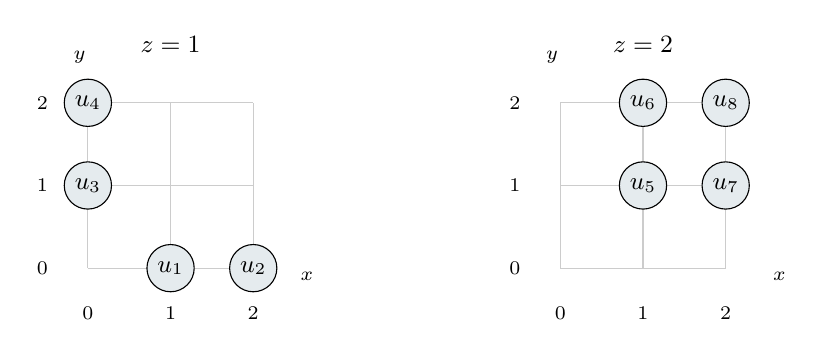
\begin{tikzpicture}[x=1.05cm,y=1.05cm]
\foreach \offset/\z in {0/1,6/2} {
 \begin{scope}[xshift=\offset cm]
 \draw[step=1,gray!40,thin] (0,0) grid (2,2);
 \foreach \t in {0,1,2} {
   \node[font=\scriptsize] at (\t,-.55) {$\t$};
   \node[font=\scriptsize] at (-.55,\t) {$\t$};}
 \node[font=\small] at (1,2.7) {$z=\z$};
 \node[font=\scriptsize] at (2.65,-.1) {$x$};
 \node[font=\scriptsize] at (-.1,2.55) {$y$};
 \end{scope}}
\foreach \x/\y/\i in {1/0/1,2/0/2,0/1/3,0/2/4} {
 \node[token,fill=inkblue!12] at (\x,\y) {$u_\i$};}
\begin{scope}[xshift=6cm]
\foreach \x/\y/\i in {1/1/5,1/2/6,2/1/7,2/2/8} {
 \node[token,fill=inkblue!12] at (\x,\y) {$u_\i$};}
\end{scope}
\end{tikzpicture}
\caption{The explicit core in~\eqref{eq:core}, drawn in its two nonempty
coordinate layers. The grid records coordinates, not affine incidence;
finite-field lines also wrap modulo $3$. There are no core points at $z=0$.}
\label{fig:core}
\end{figure}

\begin{figure}[htbp]
\centering
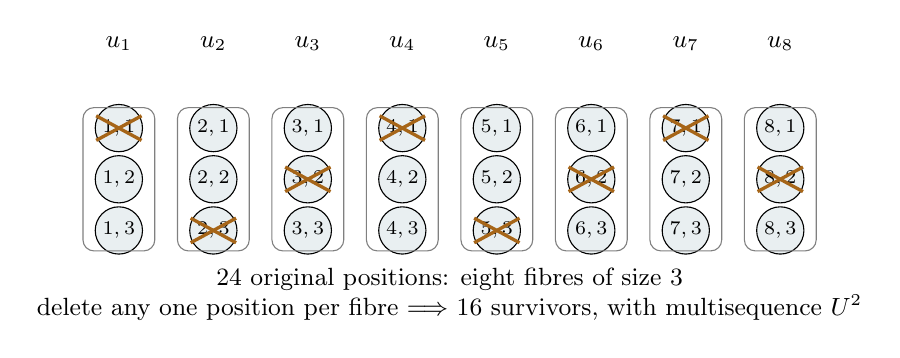
\begin{tikzpicture}[x=1.2cm,y=.65cm]
\foreach \i in {1,...,8} {
 \node[font=\small] at (\i,.65) {$u_\i$};
 \foreach \j in {1,2,3} {
  \node[token,fill=inkblue!10] (t\i\j) at (\i,-\j) {\scriptsize $\i,\j$};}
 \draw[gray,rounded corners] (\i-.38,-3.4) rectangle (\i+.38,-.6);
}
\foreach \i/\j in {1/1,2/3,3/2,4/1,5/3,6/2,7/1,8/2} {
 \draw[warm,very thick] (\i-.24,-\j-.24)--(\i+.24,-\j+.24);
 \draw[warm,very thick] (\i-.24,-\j+.24)--(\i+.24,-\j-.24);
}
\node[align=center,font=\small] at (4.5,-4.25)
 {$24$ original positions: eight fibres of size $3$\\
 delete any one position per fibre $\Longrightarrow$ $16$ survivors, with multisequence $U^2$};
\end{tikzpicture}
\caption{The positional form of $U^3$. Every column is one short zero-sum
witness. The marked representatives illustrate one of $3^8$ possible
deletions; every choice leaves the same value multiplicities.}
\label{fig:fibres}
\end{figure}

\begin{example}[A sharpness check and a length-$15$ residual]\label{ex:residual}
For the explicit $U$ above, $\sig(U)=0$: each coordinate sum is divisible
by $3$. The short-free sequence $R=U^2u_1^{-1}$ has multiplicities
$1,2,2,2,2,2,2,2$ and sum $-u_1=(2,0,2)$.
Its unique singleton $u_1$ is therefore $-\sig(R)$, illustrating
Lemma~\ref{lem:fifteen} below. The sequence $U^3u_1$, of length $25$,
fails~\eqref{eq:avoid} by the two overlapping triples on its four $u_1$
positions, exactly as in Example~\ref{ex:four}.
\end{example}
\FloatBarrier

\section{Atom packing and the four signatures}\label{sec:packing}
We now prove necessity. Throughout Sections~\ref{sec:packing}--\ref{sec:nine},
$S=(a_p)_{p\in P}$ has $24$ nonzero entries and satisfies~\eqref{eq:avoid}.
A nonempty zero-sum sequence is an \emph{atom} if it has no proper nonempty
zero-sum subsequence.

\begin{lemma}[Disjointness of distinct witnesses]\label{lem:disjoint}
Every short zero-sum witness in a sequence over $G\setminus\{0\}$ is
an atom of size $2$ or $3$. If the sequence satisfies~\eqref{eq:avoid},
any two distinct short zero-sum witnesses are disjoint.
\end{lemma}
\begin{proof}
A witness cannot be a singleton. A two-term witness is minimal.
A three-term witness cannot contain a zero-sum pair, since its remaining
entry would then be zero, so it too is minimal.
If witnesses $I,J$ intersect nontrivially,~\eqref{eq:avoid} makes their
intersection a nonempty zero-sum subset of each. Minimality implies
$I=I\cap J=J$.
\end{proof}

Choose a maximal family of pairwise position-disjoint short atoms, and
write the corresponding positional decomposition as
\begin{equation}\label{eq:packing}
 S=B_1\cdots B_l B_{l+1}\cdots B_s S_0,
 \qquad |B_i|=\begin{cases}3&i\leq l,\\2&i>l.\end{cases}
\end{equation}
Here $r=|S_0|$, and maximality means that the remaining positions $S_0$
contain no short zero sum. Such a packing exists because $P$ is finite.
In fact Lemma~\ref{lem:disjoint} shows that every short witness is a packed
block: otherwise it would be disjoint from all the blocks and could be added.
This observation makes the universal choice in the following published
deletion method explicit.

\begin{lemma}[Universal representative deletion]\label{lem:delete}
For every choice of a position $p_i$ in each $B_i$, write $x_i=a_{p_i}$.
Then
\begin{align}
 R_x&=S(x_1\cdots x_s)^{-1} &&\text{is short-free},\label{eq:all-delete}\\
 Q_x&=S(x_1\cdots x_l)^{-1} &&\text{has no three-term zero sum}.
 \label{eq:triple-delete}
\end{align}
\end{lemma}
\begin{proof}
Any short witness in $R_x$ would be a short witness in $S$, hence would
be one of the $B_i$. But each $B_i$ has lost a position.
Likewise a three-term witness in $Q_x$ would be one of
$B_1,\ldots,B_l$, each of which has lost a position.
The argument did not restrict the selected representatives.
\end{proof}

Lemma~\ref{lem:delete} is the representative-deletion argument from the
proof of \cite[Lemma 3.3(3)]{Gao2024}, applied before using any threshold
length assumption. Its universal quantifier is essential: the proof below
compares different transversals of the same fixed packing.

\begin{proposition}[Four possibilities]\label{prop:four}
Every packing~\eqref{eq:packing} has one of the signatures
\begin{equation}\label{eq:four}
 (l,s,r)\in\{(6,8,2),(7,8,1),(8,8,0),(6,9,0)\}.
\end{equation}
\end{proposition}
\begin{proof}
By Proposition~\ref{prop:inputs} and Lemma~\ref{lem:delete},
\[
          24-l=|Q_x|\leq18,\qquad 24-s=|R_x|\leq16.
\]
Thus $l\geq6$ and $s\geq8$. Length accounting gives
\begin{equation}\label{eq:budget}
        24=3l+2(s-l)+r=l+2s+r,\qquad l\leq s,\quad r\geq0.
\end{equation}
It follows that $s\leq9$. If $s=8$, then $l+r=8$, so
$(l,r)=(6,2),(7,1)$ or $(8,0)$. If $s=9$, then $l+r=6$;
hence $(l,r)=(6,0)$.
\end{proof}

\begin{figure}[htbp]
\centering
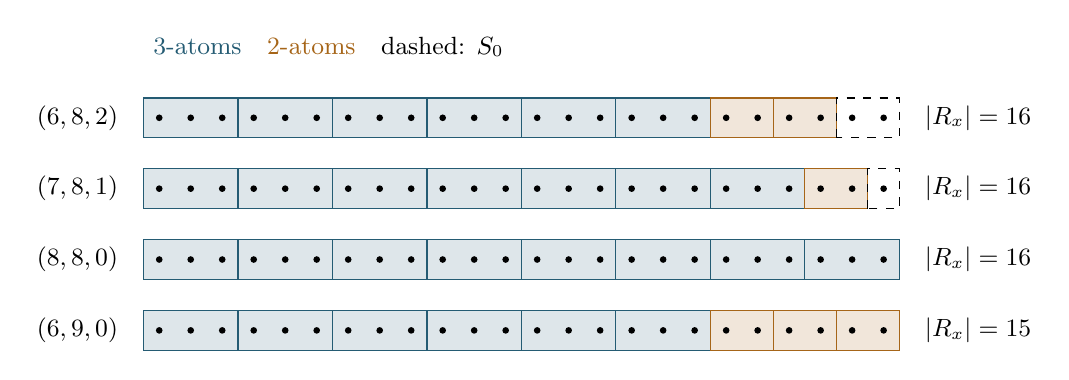
\begin{tikzpicture}[x=.40cm,y=.9cm]
\foreach \l/\s/\r/\yy in {6/8/2/0,7/8/1/-1,8/8/0/-2,6/9/0/-3} {
 \node[anchor=east,font=\small] at (-.5,\yy) {$(\l,\s,\r)$};
 \foreach \b in {1,...,\l} {
  \pgfmathtruncatemacro{\start}{3*(\b-1)}
  \filldraw[fill=inkblue!15,draw=inkblue] (\start,\yy-.28) rectangle (\start+3,\yy+.28);
  \foreach \k in {1,2,3} {\fill (\start+\k-.5,\yy) circle (1.2pt);}}
 \pgfmathtruncatemacro{\npairs}{\s-\l}
 \ifnum\npairs>0
 \foreach \b in {1,...,\npairs} {
  \pgfmathtruncatemacro{\start}{3*\l+2*(\b-1)}
  \filldraw[fill=warm!16,draw=warm] (\start,\yy-.28) rectangle (\start+2,\yy+.28);
  \foreach \k in {1,2} {\fill (\start+\k-.5,\yy) circle (1.2pt);}}
 \fi
 \ifnum\r>0
 \pgfmathtruncatemacro{\start}{\l+2*\s}
 \draw[dashed] (\start,\yy-.28) rectangle (24,\yy+.28);
 \foreach \k in {1,...,\r} {\fill (\start+\k-.5,\yy) circle (1.2pt);}
 \fi
 \pgfmathtruncatemacro{\res}{24-\s}
 \node[anchor=west,font=\small] at (24.5,\yy) {$|R_x|=\res$};}
\node[anchor=west,font=\small] at (0,1) {\textcolor{inkblue}{3-atoms}\quad
\textcolor{warm}{2-atoms}\quad dashed: $S_0$};
\end{tikzpicture}
\caption{All four length budgets. Each dot is an original position;
each solid box is a zero-sum block. These are candidate signatures under
the hypothesis, not asserted examples. Only the third row survives.}
\label{fig:packing}
\end{figure}

\section{Length-16 survivors force constant blocks}\label{sec:eight}
\begin{proposition}\label{prop:eight}
If $s=8$, then $(l,s,r)=(8,8,0)$ and every $B_i$ is a constant
three-term sequence. The sequence has the form $U^3$ for a squarefree
short-free $U$ of length $8$.
\end{proposition}
\begin{proof}
For every transversal $x$, Lemma~\ref{lem:delete} gives a short-free
$R_x$ of length $16$. Proposition~\ref{prop:inputs}(2) therefore gives
\begin{equation}\label{eq:zero-residual}
                  \sig(S)-\sum_{i=1}^8x_i=0.
\end{equation}
Fix a block $B_j$ and fix the representative positions in all other
blocks. Let $t$ be the sum of their values. If two positions in $B_j$
have values $a,b$, applying~\eqref{eq:zero-residual} with each choice gives
\[
               \sig(S)-t-a=0=\sig(S)-t-b.
\]
Hence $a=b$. All entries within every packed block are equal.

A constant two-term block would have sum $2a=0$, which forces $a=0$
in $G$, contrary to the alphabet. Thus there are no two-term blocks.
The first two signatures in~\eqref{eq:four} are excluded, leaving
$(8,8,0)$. Write $B_i=u_i^3$ and $U=u_1\cdots u_8$.
Deleting any one position from each block leaves $U^2$, which is
short-free. If $u_i=u_j$ for $i\neq j$, then $U^2$ would contain at
least four copies of this value and hence a zero-sum triple.
Therefore $U$ is squarefree. Being a subsequence of $U^2$, it is also
short-free.
\end{proof}

\begin{example}[What the representative swap compares]\label{ex:swap}
If a hypothetical two-term packed block has values $a,-a$, keep all
other deletions fixed and denote the other $15$ survivors by $W$.
The two residuals are $W(-a)$ and $Wa$. When $s=8$, both have length
$16$, so both must have sum zero. Their sum difference is $2a\neq0$,
which is impossible. For a three-term block the same comparison forces
any two selectable values to agree. The comparison concerns two
deletions of one sequence, without assuming that a preferred deletion
represents every transversal.
\end{example}
\FloatBarrier

\section{Length-15 survivors exclude nine blocks}\label{sec:nine}
\subsection{The unique singleton}
We record the precise residual fact needed for exchanges. Its multiplicity
and completion reasoning follows
\cite[proof of Lemma 27(3), together with Lemma 28]{Fan2012}.
We include the details to identify the singleton in each positional residual.

\begin{lemma}\label{lem:fifteen}
Every short-free length-$15$ sequence $R$ over $G\setminus\{0\}$ has
exactly eight support values, seven of multiplicity two and one of
multiplicity one. If $u$ is the singleton value, then
\begin{equation}\label{eq:singleton}
                         u=-\sig(R).
\end{equation}
In particular $\sig(R)\neq0$.
\end{lemma}
\begin{proof}
Every multiplicity is at most two, since $a^3$ has sum zero. Thus at
least eight values occur. Choosing one copy of every support value
produces a squarefree short-free sequence, whose length is at most eight
by Lemma~\ref{lem:double}. Exactly eight values occur, and their positive
multiplicities sum to $15$, giving the profile $2^7 1$.

Let $T$ be the squarefree support sequence. Appending the singleton $u$
gives $Ru=T^2$, which is short-free by Lemma~\ref{lem:double} and has
length $16$. Proposition~\ref{prop:inputs}(2) now yields
$0=\sig(Ru)=\sig(R)+u$. Finally $u\neq0$.
\end{proof}

\subsection{The two possible multiplicity exchanges}
Suppose the last signature in~\eqref{eq:four}, $(l,s,r)=(6,9,0)$,
occurs. All positions belong to zero-sum blocks, so $\sig(S)=0$.
For every transversal $x=(x_1,\ldots,x_9)$, the residual $R_x$ is
short-free of length $15$, with unique singleton value
\begin{equation}\label{eq:singleton-transversal}
              u_x=-\sig(R_x)=\sum_{i=1}^9 x_i.
\end{equation}

Fix a block $B_j$ with two distinct selectable values $a\neq b$.
Fix representatives in the other eight blocks, with value-sum $t$.
Let $R_a$ and $R_b$ be the residuals obtained by deleting the chosen
position of value $a$ and of value $b$, respectively. The choices are
distinct positions in the same block. As multisets of values,
\begin{equation}\label{eq:exchange}
                         R_b=R_a\,a\,b^{-1}.
\end{equation}
The removed copy of $b$ is present in $R_a$, so this equation is legitimate.

\begin{lemma}\label{lem:exchange}
For fixed complementary representatives as above, the counts
$(v_a(R_a),v_b(R_a))$ and $(v_a(R_b),v_b(R_b))$ must follow exactly one
of the transitions
\begin{equation}\label{eq:transitions}
             (0,1)\longmapsto(1,0),\qquad
             (1,2)\longmapsto(2,1).
\end{equation}
The first transition is impossible under~\eqref{eq:singleton-transversal};
the second forces $t=0$.
\end{lemma}
\begin{proof}
By~\eqref{eq:exchange}, the count of $a$ increases by one and that of
$b$ decreases by one. All counts in each residual lie in $\{0,1,2\}$,
and exactly one value has count one. Initially the count of $a$ is
$0$ or $1$, and that of $b$ is $1$ or $2$.
The possibility $(1,1)$ already gives two singletons. The possibility
$(0,2)$ becomes $(1,1)$ and gives two singletons after the exchange.
The two remaining possibilities are~\eqref{eq:transitions}.

In the first case the singleton of $R_a$ is $b$, and that of $R_b$ is
$a$. Equation~\eqref{eq:singleton-transversal} gives
\[
                      b=t+a,\qquad a=t+b.
\]
Subtracting these equations gives $2(a-b)=0$, hence $a=b$ since
multiplication by two is invertible in $G$. This is a contradiction.

In the second case the singletons of $R_a,R_b$ are $a,b$, respectively.
Their identities give
\[
                     a=t+a,\qquad b=t+b,
\]
and therefore $t=0$.
\end{proof}

\begin{figure}[htbp]
\centering
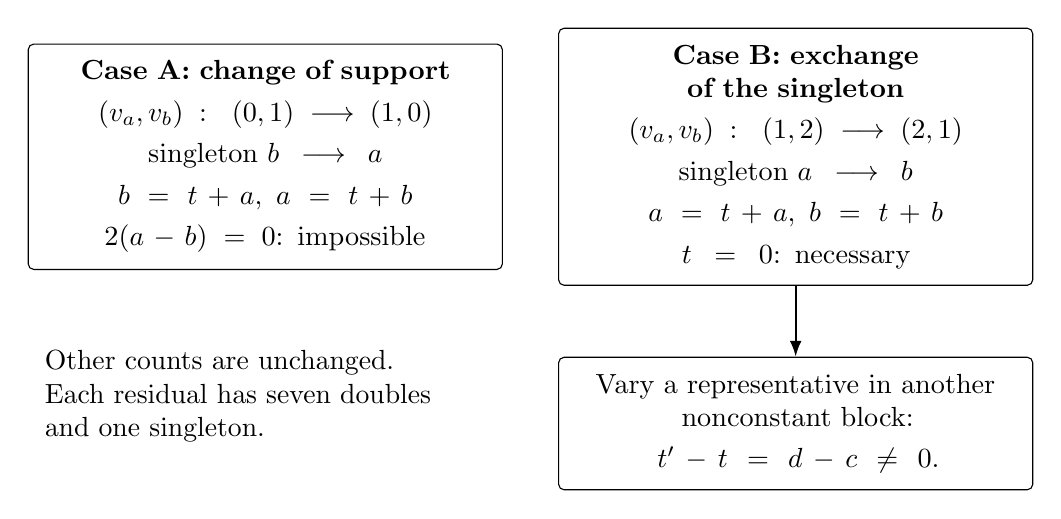
\begin{tikzpicture}[x=1cm,y=1cm]
\node[box,text width=5.6cm] (case1) at (0,0)
 {\textbf{Case A: change of support}\\[3pt]
 $(v_a,v_b):\ (0,1)\longrightarrow(1,0)$\\[3pt]
 singleton $b\longrightarrow a$\\[3pt]
 $b=t+a,\ a=t+b$\\[3pt]
 $2(a-b)=0$: impossible};
\node[box,text width=5.6cm,right=7mm of case1] (case2)
 {\textbf{Case B: exchange of the singleton}\\[3pt]
 $(v_a,v_b):\ (1,2)\longrightarrow(2,1)$\\[3pt]
 singleton $a\longrightarrow b$\\[3pt]
 $a=t+a,\ b=t+b$\\[3pt]
 $t=0$: necessary};
\node[box,below=9mm of case2,text width=5.6cm] (other)
 {Vary a representative in another\\ nonconstant block:\\[3pt]
 $t'-t=d-c\neq0$.};
\draw[flow] (case2)--(other);
\node[align=left,text width=5.6cm,below=9mm of case1]
 {Other counts are unchanged.\\
 Each residual has seven doubles\\ and one singleton.};
\end{tikzpicture}
\caption{The exhaustive exchange in a hypothetical nine-block packing.
Case A contradicts $a\neq b$. Case B requires zero complementary sum
for every choice, which another nonconstant block makes impossible.}
\label{fig:exchange}
\end{figure}

\begin{proposition}\label{prop:nine}
The signature $(6,9,0)$ cannot occur.
\end{proposition}
\begin{proof}
It has three two-term zero-sum blocks. Each has distinct values $a,-a$:
if they were equal, $2a=0$ would contradict $a\neq0$.
Choose one as $B_j$. For \emph{every} choice of representatives in the
other eight blocks, Lemma~\ref{lem:exchange} forces their sum $t$ to be
zero. Choose a second two-term block $B_k$, $k\neq j$, whose distinct
values are $c,d$. Keep the remaining seven representatives fixed and
let their sum be $h$. Choosing $c$ and then $d$ in $B_k$ gives
\[
                           h+c=0=h+d.
\]
Thus $c=d$, a contradiction.
\end{proof}

\begin{example}[The profile exchange is not itself a contradiction]\label{ex:local}
For distinct $a,b$, the abstract profiles
$a b^2 c_1^2\cdots c_6^2$ and $a^2 b c_1^2\cdots c_6^2$
both have length $15$ and shape $2^7 1$. They illustrate the second
transition; they are not asserted to be short-free sequences.
The obstruction uses the singleton \emph{sums} as well as the counts,
and then varies a representative in a different block.
This separates the local multiplicity comparison from the global
nine-block contradiction.
\end{example}
\FloatBarrier

\section{Completion of the classification}\label{sec:completion}
\begin{proof}[Proof of Theorem~\ref{thm:main}]
Assume~(1). Proposition~\ref{prop:four} supplies the four signatures.
Proposition~\ref{prop:nine} excludes $s=9$; Proposition~\ref{prop:eight}
then leaves eight constant three-position blocks with distinct values
$u_1,\ldots,u_8$, and their squarefree core $U$ is short-free.
Number the three original positions in each block arbitrarily. Sending
$(i,j)$ to the $j$th position of block $i$ defines the bijection $\phi$
in~\eqref{eq:permutation}. This explicitly accounts for all $24$ original
positions and proves~(2).

Conversely, assume~(2), and work first on the product index set
$\{1,\ldots,8\}\times\{1,2,3\}$. There is no singleton witness.
A pair with different values would be a short zero sum in $U$, and a
pair with equal value $a$ has sum $2a\neq0$.
In a zero-sum triple, three distinct values would again give a short
zero sum in $U$. If a value $a$ repeats, $2a+b=0$ implies $b=a$.
The witness is therefore exactly the full three-position fibre of $a$,
since there are only three positions with that value.

Consequently any two short witnesses are either identical fibres, whose
intersection has sum $3a=0$, or different fibres, whose intersection is
empty. The bijection $\phi$ preserves intersections and all entry sums:
for position sets $I,J$,
$\phi^{-1}(I\cap J)=\phi^{-1}(I)\cap\phi^{-1}(J)$.
Transporting the conclusion proves~\eqref{eq:avoid} on the original $P$.
This is a direct positional verification of the already known
construction from \cite[proof of Lemma 3.3(2)]{Gao2024}.
\end{proof}

\begin{corollary}\label{cor:witnesses}
Every length-$24$ sequence satisfying~\eqref{eq:avoid} has exactly eight
short zero-sum witnesses. They are disjoint constant triples and partition
the original position set. Every support value has multiplicity three.
\end{corollary}
\begin{proof}
The last part of the proof of Theorem~\ref{thm:main} identifies all witnesses
as the eight full value fibres. Each such fibre is a witness.
\end{proof}

\section{Discussion and formal verification}
\subsection{The inverse content}
Theorem~\ref{thm:main} complements the published threshold by determining
every multiplicity and every short witness in every extremal sequence.
At residual length $16$, fixed total sum forces equal entries within
blocks. At length $15$, the singleton identity couples independently
variable representatives, excluding the competing packing.
These deductions supply the necessity beyond the known construction.
The argument uses specific rank-three residual facts and no enumeration
of extremal sequences. We make no assertion for other ranks, exponents
or lengths. Nor do we claim a new core classification: the core normal
form in \cite[Lemma 9]{Fan2012} is prior work.

\subsection{A geometric interpretation of the core}
After the multiplicity conclusion has been proved, the core may be viewed
as a set of eight points. Adjoining $0$ gives a nine-point cap in
$\operatorname{AG}(3,3)$: three distinct points in characteristic three
are collinear exactly when their sum is zero. A line through $0$
corresponds to a forbidden pair $a,-a$ in $U$, and a line not through
$0$ corresponds to a forbidden distinct triple in $U$.
This explains the core in Figure~\ref{fig:core}; it does not supply the
necessity of the threefold multiplicities on the original positions.

\subsection{Formal statement and provenance}
The positional equivalence of Theorem~\ref{thm:main} has a Lean
formalization, registered as
\href{https://palomar-registry.org/entry.html?id=PALOMAR-2026-10-09-000011&version=1}{PALOMAR-2026-10-09-000011, version 1}~\cite{Palomar2026}.
The declaration is:
\begin{center}\small\ttfamily
InverseZeroSum.Candidate3.frozenClassification
\end{center}
It uses $\operatorname{Fin}(24)$ positions, nonzero entries, finite position
sets for witnesses, and an explicit permutation for threefold repetition.
Both implications and the required source-input propositions are proved.
The registration supplies the immutable source revision, using Lean
\texttt{4.35.0-rc2}. Formal registration concerns the encoded theorem;
the exposition and source attributions above stand separately.

\paragraph{AI assistance.}
OpenAI ChatGPT was used substantively in developing the mathematical
arguments, constructing the Lean formalization, checking literature and
preparing the manuscript, examples and diagrams. Responsibility for the
article and its attributions remains with the author.

\begingroup
\small
\bibliographystyle{plain}
\bibliography{references}
\endgroup
\end{document}
